\clearpage
\section{Fixed task sets}
\label{app:fixed_populations}

A line of a mean over tasks against model size averages, at each size, the tasks that have a value there. The above-chance gate keeps more tasks at larger sizes, so a line can rise or fall because its tasks changed. Each figure below redraws a paper figure on one task set per line, the tasks that have a value at every point of that line (solid), with the original line dashed behind it.

\begin{figure*}[p]
\centering
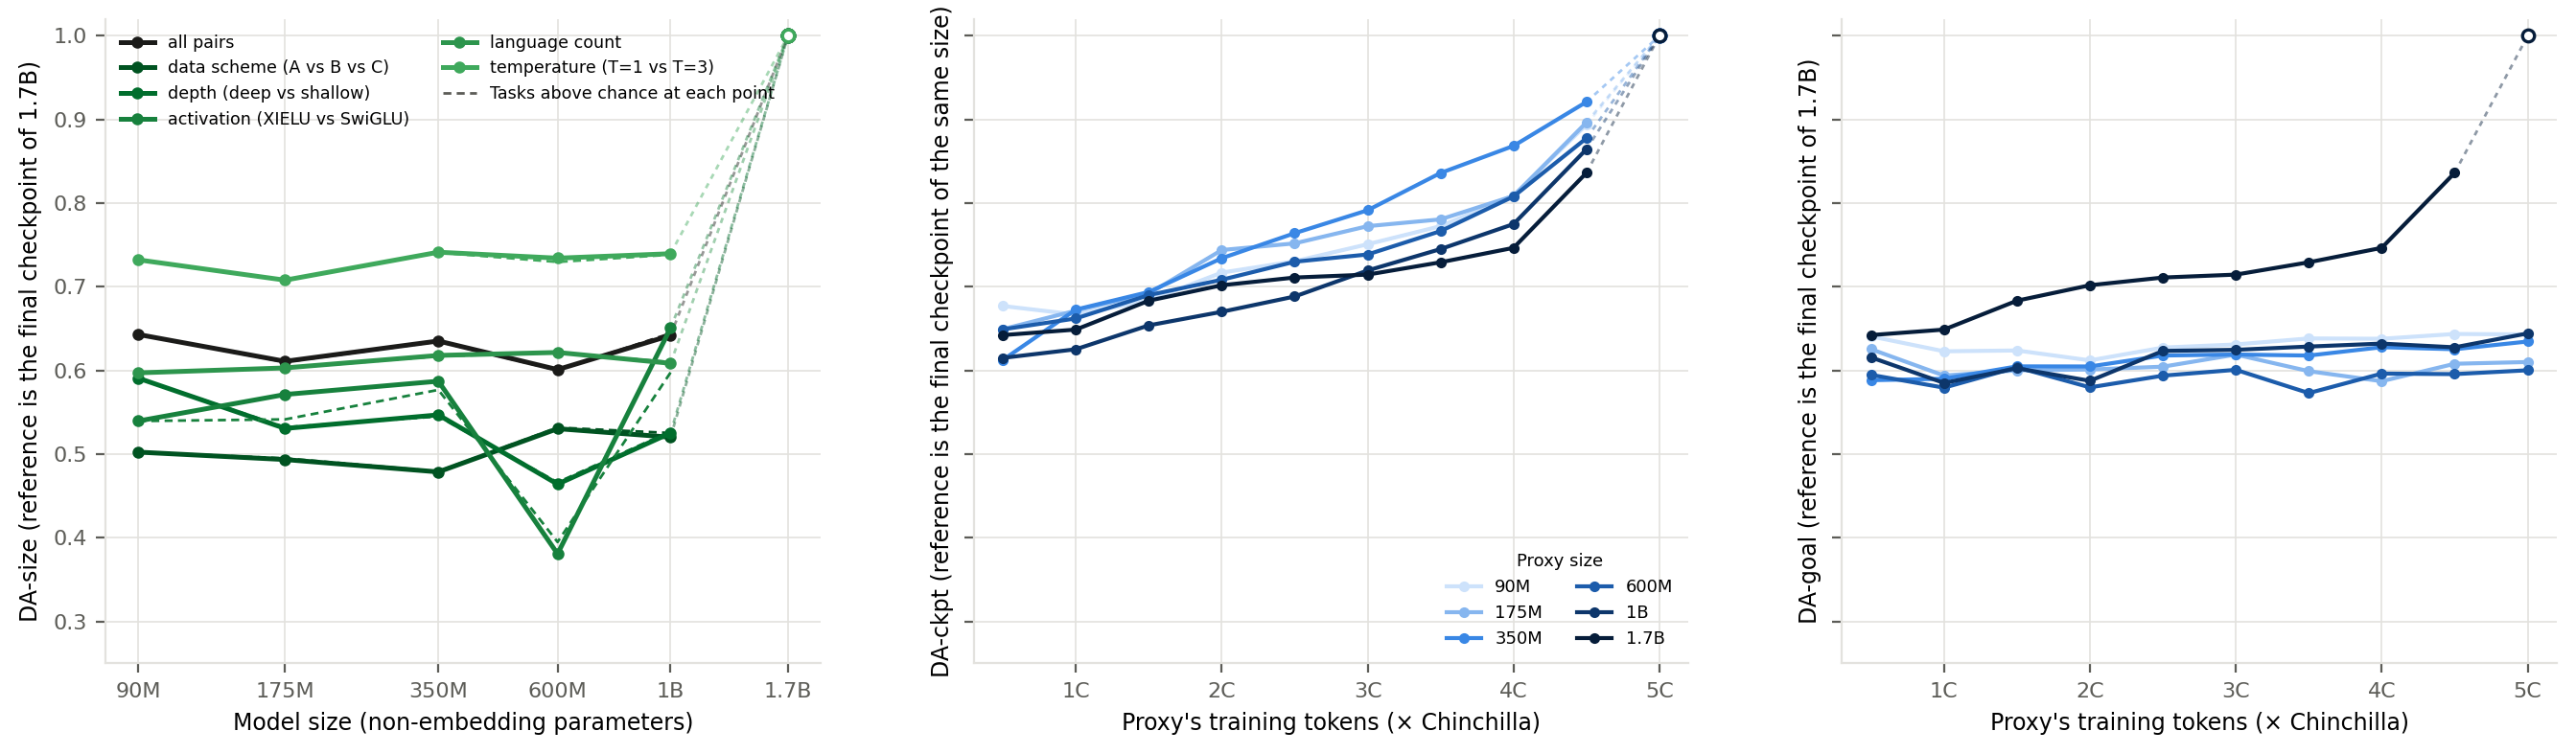
\includegraphics[width=\textwidth,height=0.8\textheight,keepaspectratio]{figures/app_rq02_fixed_rq2.png}
% source: src/signal-and-noise/analysis/rq02_decision_accuracy/pretraining/predictivity/rq2_da_all_above_66_either_transformation_mono_axis_fixed_tasks_paper.png
\caption{\textbf{Holding the tasks fixed moves the DA-size line over every single-axis pair by at most $-$0.00 (at 1B), small against the line's own range, so its shape is not a population effect.} Figure~\ref{fig:rq2} on one task set per line, the reliable tasks of each panel that have a value at every point (solid), against the original (dashed). The 690 tasks it has at every point read 0.64 at 90M and 0.64 at 1B, against 0.64 and 0.64 on the tasks of each point (690--723).}
\label{fig:app_rq02_fixed_rq2}
\end{figure*}

\begin{figure*}[p]
\centering
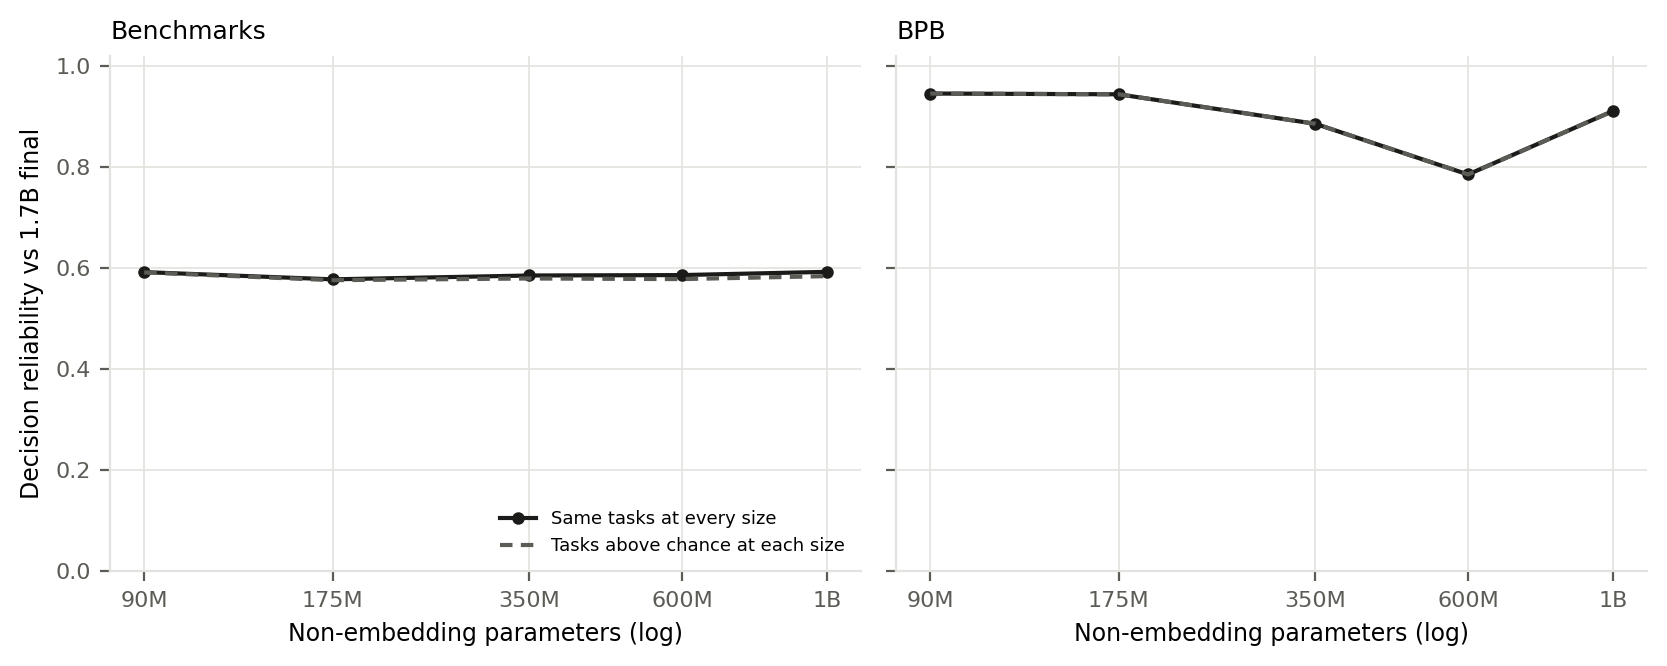
\includegraphics[width=\textwidth,height=0.8\textheight,keepaspectratio]{figures/app_rq02_fixed_decision_accuracy.png}
% source: src/signal-and-noise/analysis/rq02_decision_accuracy/pretraining/predictivity/scale_convergence_da_size_multi_axes_fixed_tasks_paper.png
\caption{\textbf{Holding the tasks fixed moves the benchmark line by at most +0.01 (at 1B), so part of the line's movement comes from its changing tasks.} Figure~\ref{fig:app_rq02_decision_accuracy} on one task set per line, the tasks above chance that have a value at every point (solid), against the original (dashed). The 1115 tasks it has at every point read 0.59 at 90M and 0.59 at 1B, against 0.59 and 0.58 on the tasks of each point (1118--1286).}
\label{fig:app_rq02_fixed_decision_accuracy}
\end{figure*}

\begin{figure*}[p]
\centering
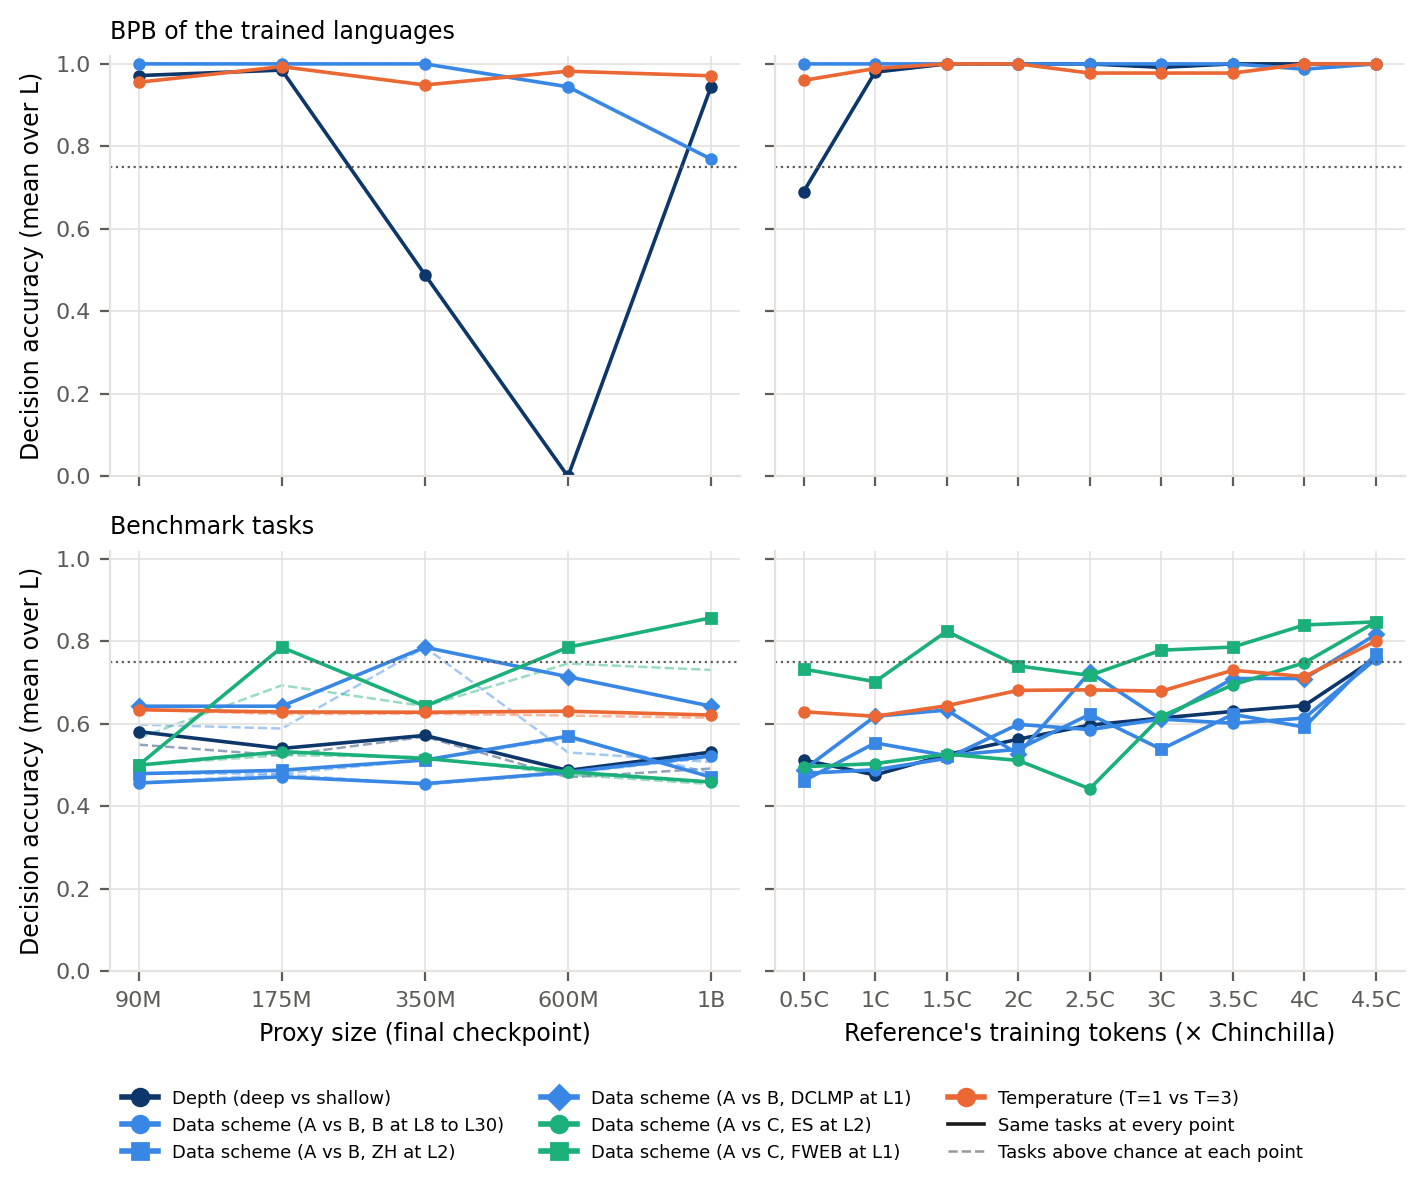
\includegraphics[width=\textwidth,height=0.8\textheight,keepaspectratio]{figures/app_rq05_fixed_design_decisions.png}
% source: src/signal-and-noise/analysis/rq05_design_decisions/pretraining/predictivity_seeds/da_all_lines_mono_axis_fixed_tasks_paper.png
\caption{\textbf{Holding the tasks fixed moves the benchmark line of the temperature decision by at most +0.01 (at 600M), so part of the line's movement comes from its changing tasks.} Figure~\ref{fig:app_rq05_design_decisions} on one task set per line, the (task, language setting) cells of each line that have a value at every point (solid), against the original (dashed). The 2502 cells it has at every point read 0.63 at 90M and 0.62 at 1B, against 0.63 and 0.61 on the cells of each point (2508--2886).}
\label{fig:app_rq05_fixed_design_decisions}
\end{figure*}

\begin{figure*}[p]
\centering
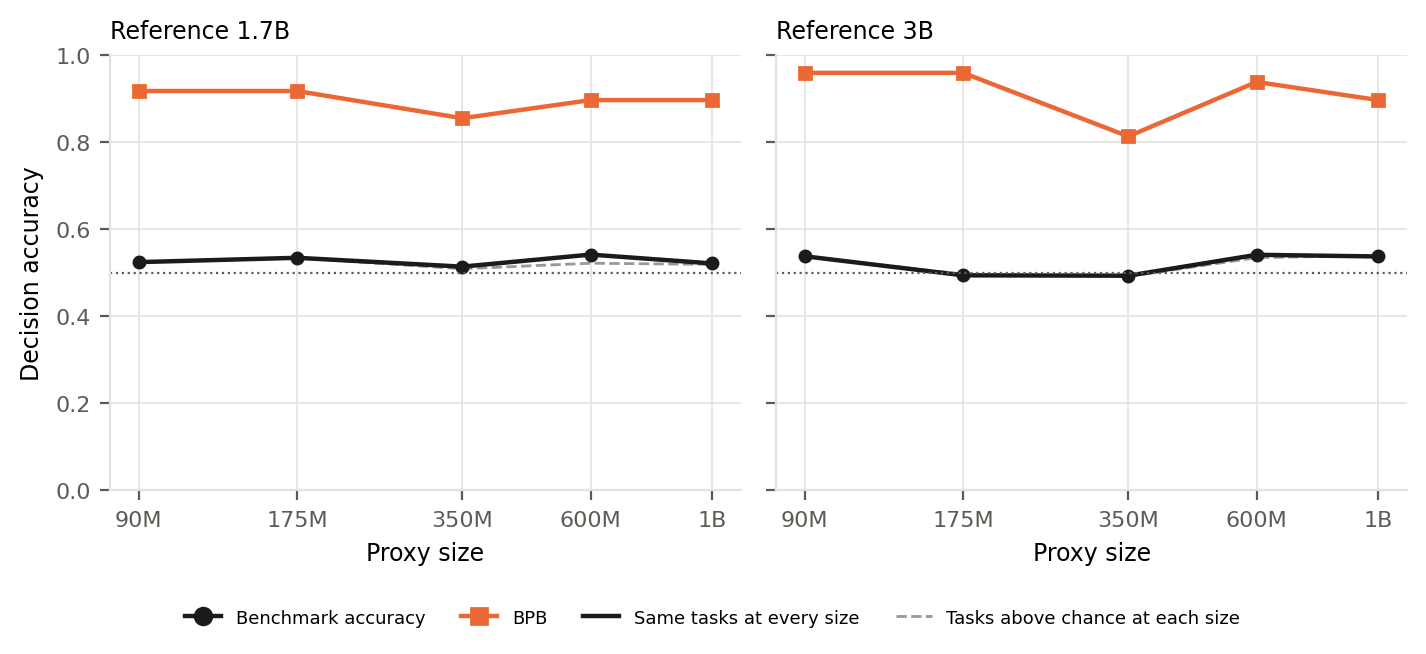
\includegraphics[width=\textwidth,height=0.8\textheight,keepaspectratio]{figures/app_rq10_fixed_size_generalisation.png}
% source: src/signal-and-noise/analysis/rq10_size_generalisation/pretraining/predictivity/gate_share_and_da_size_mono_axis_fixed_tasks_paper.png
\caption{\textbf{Holding the tasks fixed moves the benchmark line against the 3B reference by at most +0.01 (at 600M), small against the line's own range, so its shape is not a population effect.} Figure~\ref{fig:app_rq10_size_generalisation} on one task set per line, the tasks of each channel (the left panel is not redrawn) that have a value at every point (solid), against the original (dashed). The 444 tasks it has at every point read 0.54 at 90M and 0.54 at 1B, against 0.54 and 0.54 on the tasks of each point (446--536).}
\label{fig:app_rq10_fixed_size_generalisation}
\end{figure*}

\begin{figure*}[p]
\centering
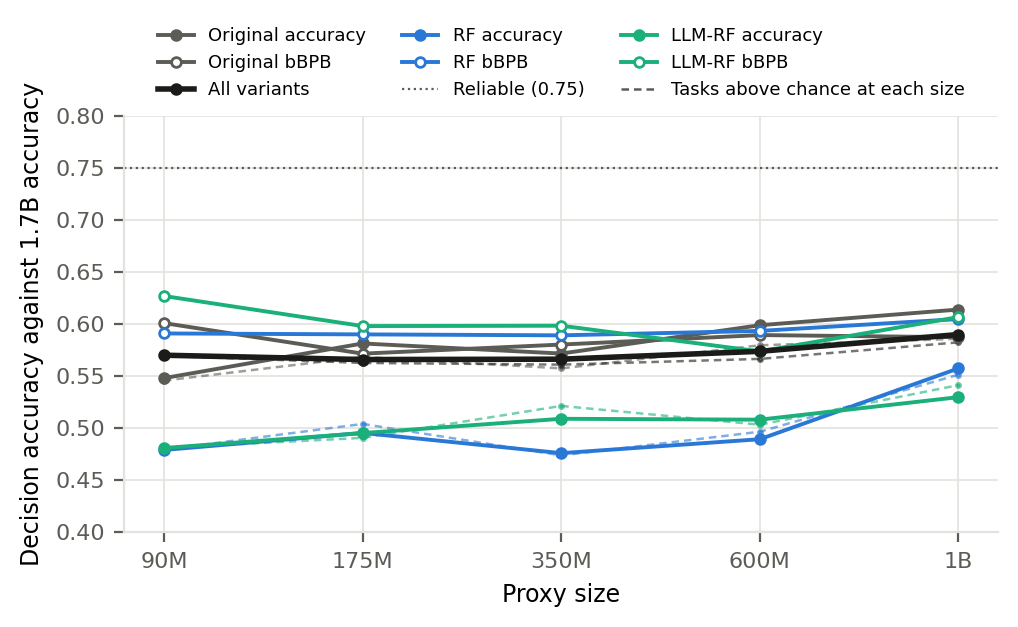
\includegraphics[width=\textwidth,height=0.8\textheight,keepaspectratio]{figures/app_rq11_fixed_evaluation_recipe.png}
% source: src/signal-and-noise/analysis/rq11_evaluation_recipe/pretraining/predictivity/recipe_da_size_variants_multi_axes_fixed_tasks_paper.png
\caption{\textbf{Holding the tasks fixed moves the pooled line by at most +0.01 (at 1B), so part of the line's movement comes from its changing tasks.} Figure~\ref{fig:app_rq11_evaluation_recipe} on one task set per line, the tasks of each variant that have a value at every point (solid), against the original (dashed). The 800 tasks it has at every point read 0.57 at 90M and 0.59 at 1B, against 0.57 and 0.58 on the tasks of each point (803--971).}
\label{fig:app_rq11_fixed_evaluation_recipe}
\end{figure*}

\begin{figure*}[p]
\centering
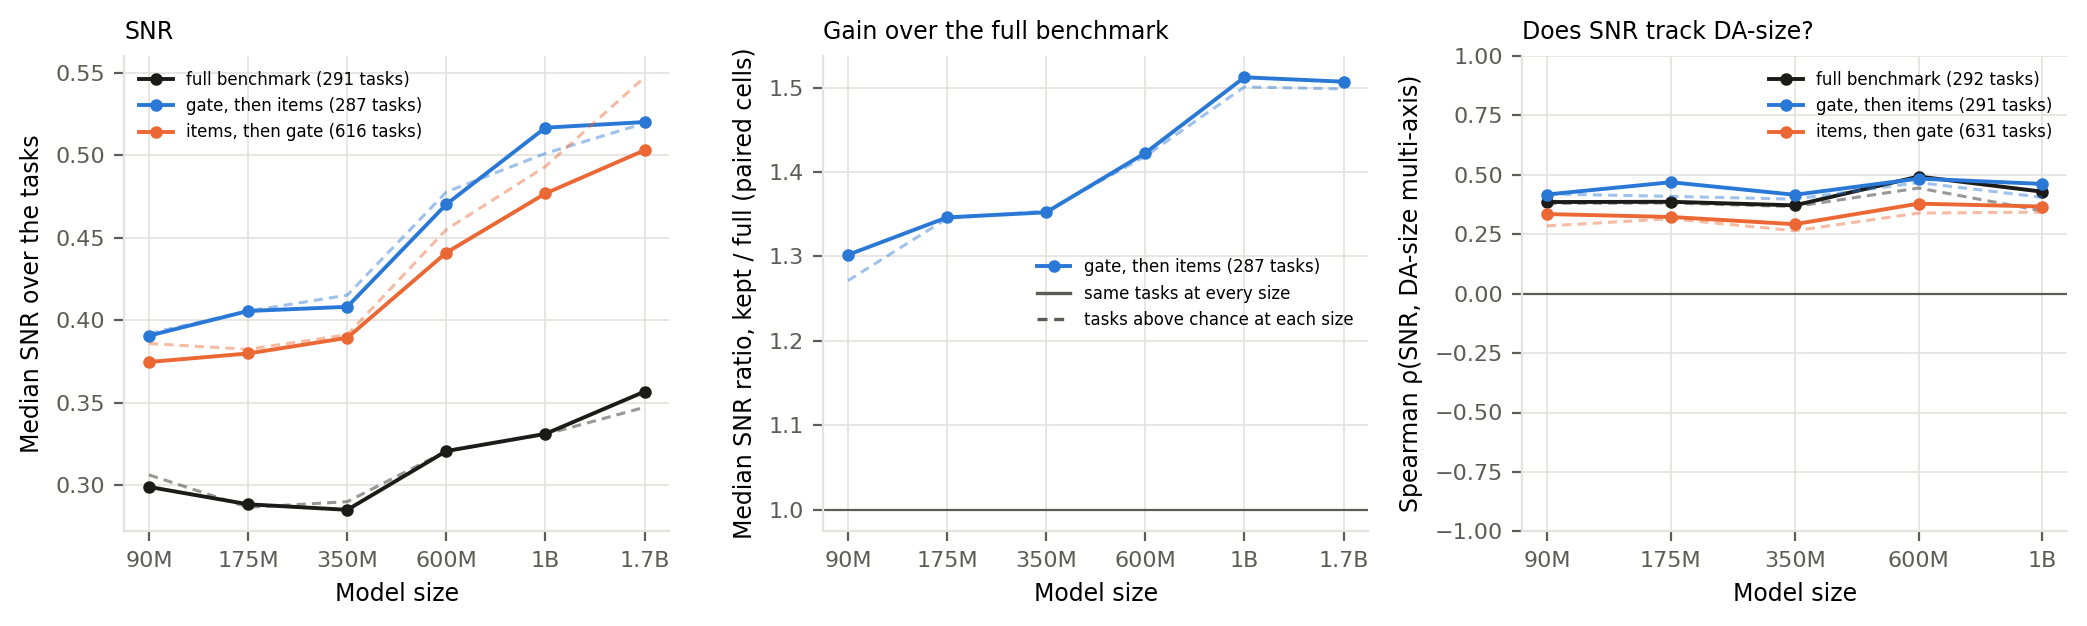
\includegraphics[width=\textwidth,height=0.8\textheight,keepaspectratio]{figures/app_rq12_fixed_above_chance_items.png}
% source: src/signal-and-noise/analysis/rq12_above_chance_items/pretraining/predictivity/above_chance_items_snr_fixed_tasks_paper.png
\caption{\textbf{Holding the tasks fixed moves the median SNR of the items-then-gate ordering by at most $-$0.04 (at 1.7B), so part of the line's movement comes from its changing tasks.} Figure~\ref{fig:app_rq12_above_chance_items} on one task set per line, the tasks of each ordering that have a value at every point (solid), against the original (dashed). The 616 tasks it has at every point read 0.37 at 90M and 0.50 at 1.7B, against 0.39 and 0.55 on the tasks of each point (676--759).}
\label{fig:app_rq12_fixed_above_chance_items}
\end{figure*}

\begin{figure*}[p]
\centering
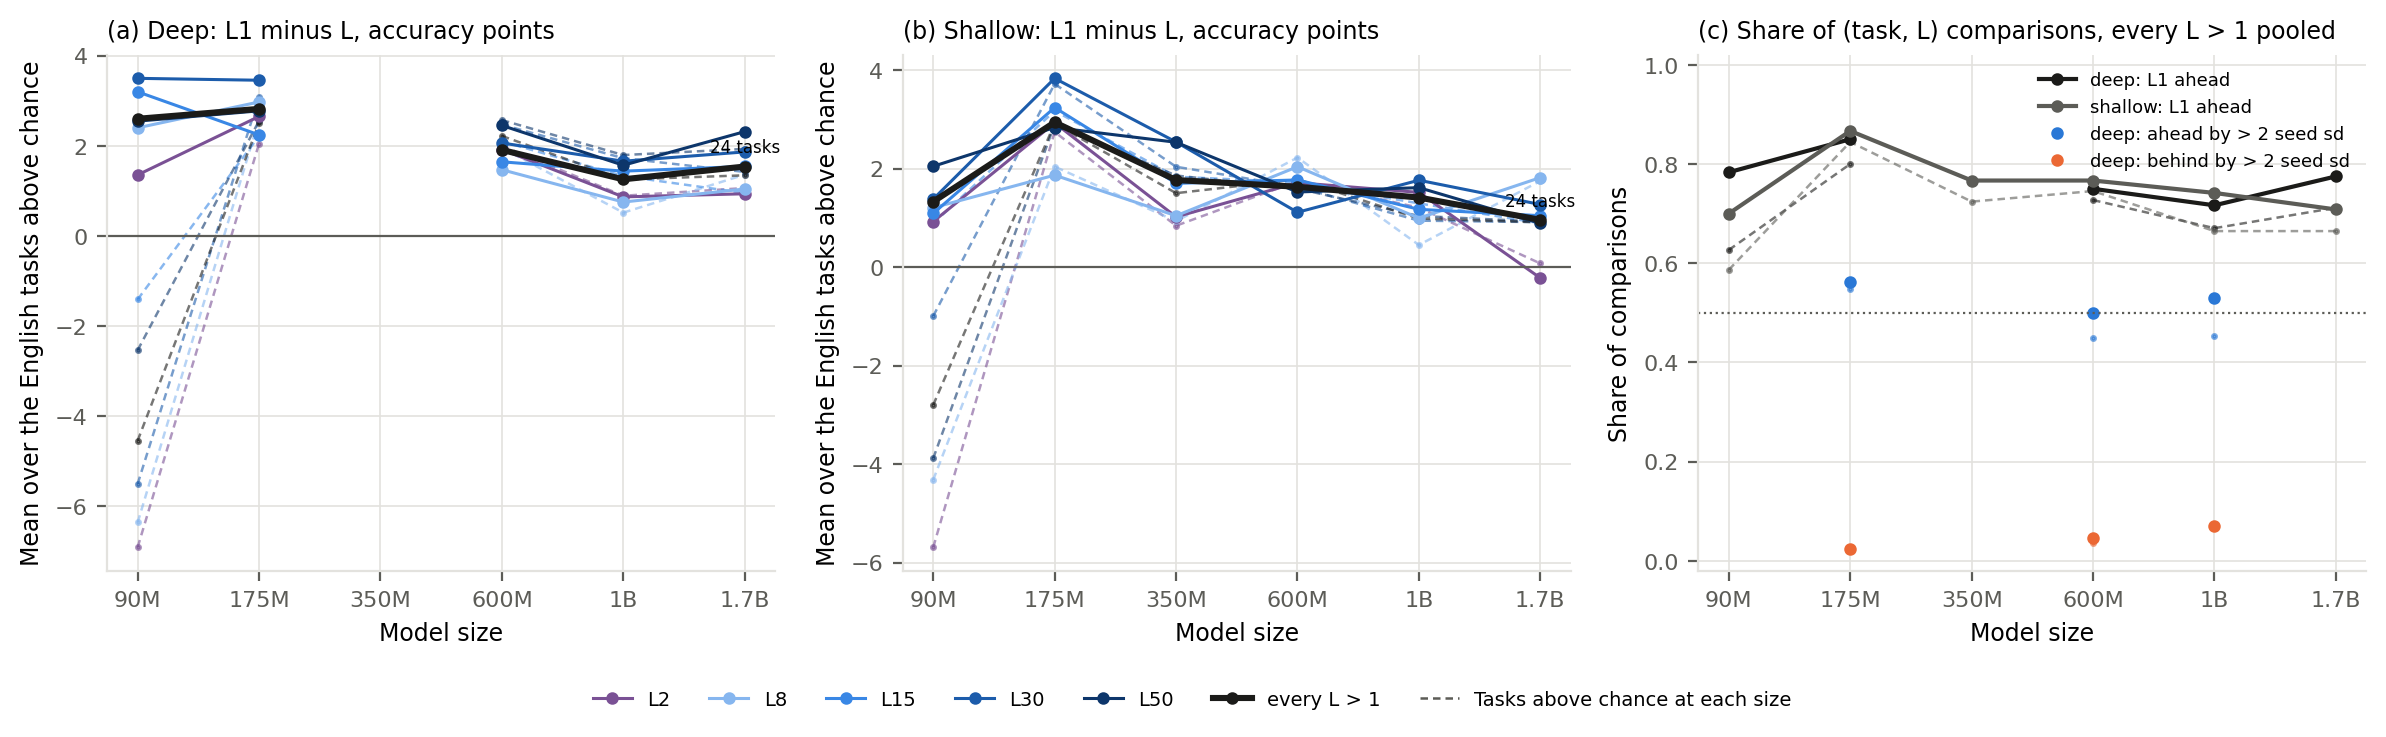
\includegraphics[width=\textwidth,height=0.8\textheight,keepaspectratio]{figures/app_rq13_fixed_english_only.png}
% source: src/signal-and-noise/analysis/rq13_english_only/pretraining/predictivity/english_only_scores_fixed_tasks_paper.png
\caption{\textbf{Holding the tasks fixed moves the deep cells' mean gap in points to every other language setting by at most +7.1 (at 90M), so part of the line's movement comes from its changing tasks.} Figure~\ref{fig:app_rq13_english_only} on one task set per line, the English tasks of each comparison that have a value at every point (solid), against the original (dashed). The 24 tasks it has at every point read 2.6 at 90M and 1.5 at 1.7B, against $-$4.5 and 1.3 on the tasks of each point (27--34).}
\label{fig:app_rq13_fixed_english_only}
\end{figure*}
